\subsubsection{Outliers}\label{sec:impl-data-analysis:outliers}
The underlying section will look into the number of outliers in the dataset. Given that the linear models, such as logistic regression one can be highly susceptible to the presence of outlying data points this part of the data analysis must be carried out.

Outliers, also referred to as residuals, are the data points not residing on a given prediction function. The magnitude of a residual is typically defined as the distance of a given data point from the proposed prediction line, in linear models.

Taking into the account the number of features present in the dataset it would be quite unfeasible to present individual box plot graphs per feature. At the same time, since the data is not yet on the same scale it would be difficult to highlight any residuals on aggregate graphs, with multiple features on each plot. Therefore it was decided that a algebraic method will be best employed instead.

The first step was to collect the following properties for each feature:
\begin{itemize}
    \item first quartile (Q1)
    \item third quartile (Q3)
    \item inter quartile range (IQR)
    \item lower boundary - value below which a data point will be considered an outlier. Set to $1.5x IQR$ below first quartile
    \item upper boundary - value above which a data point will be considered an outlier. Set to $1.5x IQR$ above third quartile
\end{itemize}

The above metrics are collected into a list. Each list item is a map of attribute to value. The information collected was then converted to a data frame for enabling easy processing. The results compiled can be observed in Tables \ref{tbl:outliers:iqr-at-0} and \ref{tbl:outliers:all-metrics}.

\begin{table}[!h]
\centering
\caption{All metrics pertaining to calculating residuals - IQR at 0}
\label{tbl:outliers:iqr-at-0}
\begin{tabular}{@{}lll@{}}
\toprule
\multicolumn{3}{c}{Feature Names} \\ \midrule
duplicated\_blocks & major\_violations & reliability\_rating \\
duplicated\_files & minor\_violations & security\_rating \\
duplicated\_lines & overall\_branch\_coverage & sqale\_debt\_ratio \\
duplicated\_lines\_density & overall\_coverage & sqale\_index \\
files & overall\_uncovered\_conditions & sqale\_rating \\
info\_violations & overall\_uncovered\_lines & test\_success\_density \\
it\_uncovered\_lines & public\_documented\_api\_density & violations \\ \bottomrule
\end{tabular}
\end{table}

\begin{table}[!h]
\centering
\caption{All metrics pertaining to calculating residuals - IQR above 0}
\label{tbl:outliers:all-metrics}
\begin{tabular}{@{}llllll@{}}
\toprule
Attribute & IQR & \begin{tabular}[c]{@{}l@{}}Lower \\ Boundary\end{tabular} & Q1 & Q3 & \begin{tabular}[c]{@{}l@{}}Upper \\ Boundary\end{tabular} \\ \midrule
classes & 1 & 0 & 0 & 1 & 2.5 \\
comment\_lines & 15 & 0 & 1 & 16 & 38.5 \\
comment\_lines\_density & 17.8 & 0 & 0.4 & 18.2 & 44.9 \\
complexity & 23 & 0 & 3 & 26 & 60.5 \\
function\_complexity & 0.7 & 0 & 1 & 1.7 & 2.75 \\
functions & 14 & 0 & 3 & 17 & 38 \\
lines\_to\_cover & 44 & 0 & 14 & 58 & 124 \\
ncloc & 105 & 0 & 32 & 137 & 294.5 \\
file\_age\_in\_sec & 87187 & 0 & 3423 & 90610 & 221390.5 \\ \bottomrule
\end{tabular}
\end{table}

Subsequently, it is checked which columns contain values above their upper outlier boundary. Another list containing the columns without residuals above such value is also compiled. 

At the end of that process it has been concluded that 22 columns contain residuals while 8 do not. Furthermore, counts of residual data points have been obtained and compiled into Table \ref{tbl:outliers:counts-original}. The items in yellow, have been highlighted to signify their $IQR$ value being above 0. From same it can be observed that the most significant numbers of residual data points is observed in \itUncoveredLines{}, closely followed by \overallUncoveredLines{}, \fileAgeInSec{} and \overallUncoveredConditions{} attributes. However, other than \fileAgeInSec{} other mentioned attributes have their $IQR$ value at 0, as per lack of the yellow highlight and given values contained in Table \ref{tbl:outliers:iqr-at-0}, meaning any data points above that value would automatically be treated as an outlier. Judging by Table \ref{tbl:outliers:all-metrics} the attributes are of similar enough scale to be grouped together for visualization, the result of which can be observed from Figures \ref{fig:outliers:boxplot-iqr-above-0-part1} and \ref{fig:outliers:boxplot-iqr-above-0-part2}. 

\begin{table}[!h]
\centering
\caption{Residual counts per feature}
\label{tbl:outliers:counts-original}
\begin{tabular}{ll}
\hline
Column & \begin{tabular}[c]{@{}l@{}}Data Points Above \\ Upper Boundary\end{tabular} \\ \hline
\rowcolor[HTML]{FFFFC7} 
classes & 534 \\
\rowcolor[HTML]{FFFFC7} 
comment\_lines & 797 \\
\rowcolor[HTML]{FFFFC7} 
comment\_lines\_density & 359 \\
\rowcolor[HTML]{FFFFC7} 
complexity & 491 \\
duplicated\_blocks & 221 \\
duplicated\_files & 221 \\
duplicated\_lines & 221 \\
duplicated\_lines\_density & 221 \\
\rowcolor[HTML]{FFFFC7} 
file\_age\_in\_sec & 985 \\
\rowcolor[HTML]{FFFFC7} 
function\_complexity & 294 \\
\rowcolor[HTML]{FFFFC7} 
functions & 462 \\
info\_violations & 11 \\
it\_uncovered\_lines & 1100 \\
\rowcolor[HTML]{FFFFC7} 
lines\_to\_cover & 652 \\
major\_violations & 70 \\
minor\_violations & 24 \\
\rowcolor[HTML]{FFFFC7} 
ncloc & 492 \\
overall\_uncovered\_conditions & 873 \\
overall\_uncovered\_lines & 1087 \\
sqale\_debt\_ratio & 96 \\
sqale\_index & 96 \\
violations & 103 \\ \hline
\end{tabular}
\end{table}

\begin{figure}[!h]
    \centering
    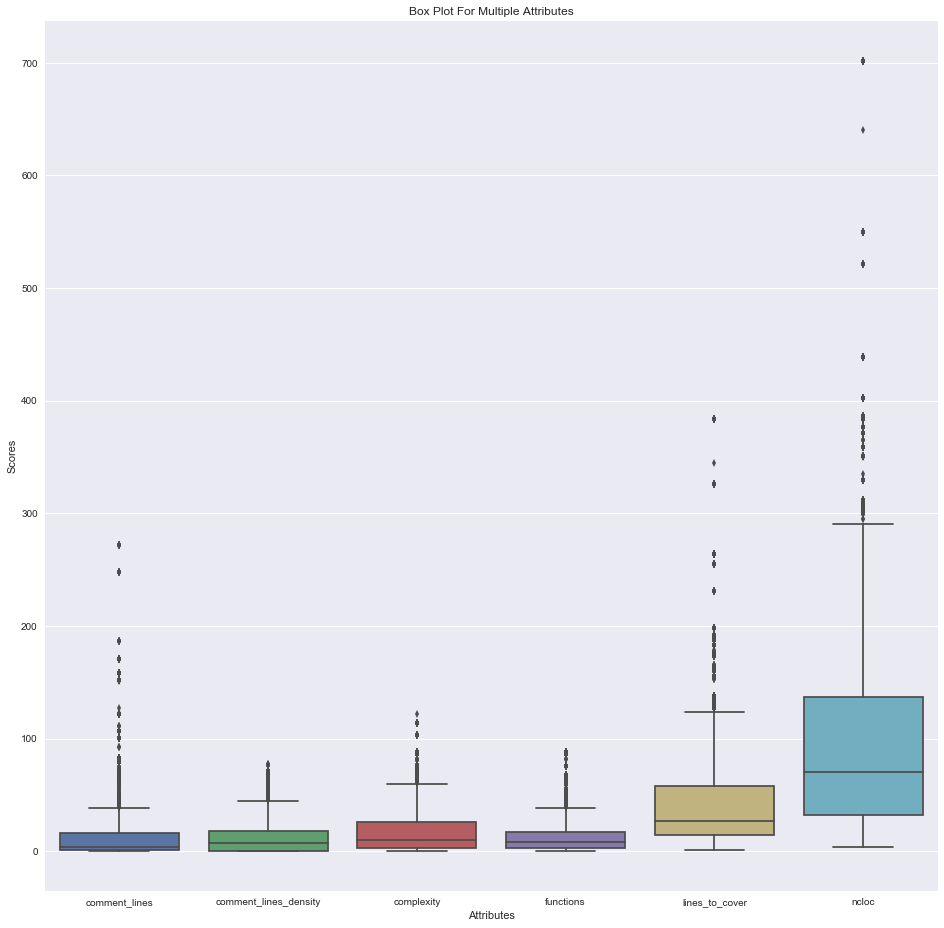
\includegraphics[scale=0.45]{Figures/boxplot_iqr_above_0_part1.png}
    \caption{Residual values for attributes with IQR > 0}
    \label{fig:outliers:boxplot-iqr-above-0-part1}
\end{figure}

\begin{figure}[!h]
    \centering
    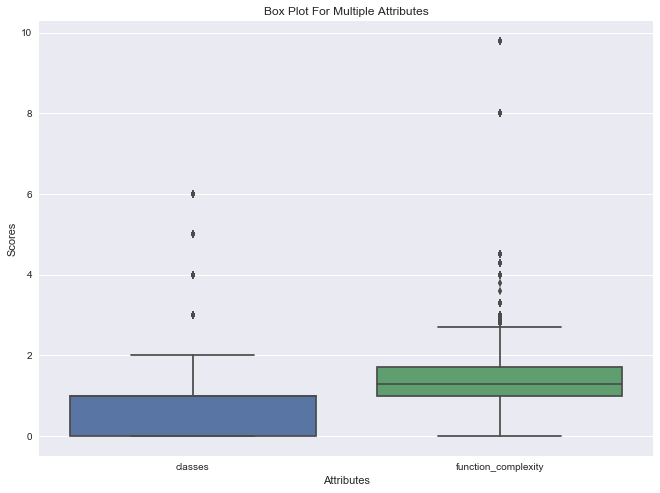
\includegraphics[scale=0.65]{Figures/boxplot_iqr_above_0_part2.png}
    \caption{Residual values for attributes with IQR > 0}
    \label{fig:outliers:boxplot-iqr-above-0-part2}
\end{figure}

\textbf{In Conclusion} it has been proven beyond any doubt that there are a number of outliers in the dataset. At this stage it has been decided against addressing the residual values as it will undergo further processing with regards to scaling as well as due to recognizing that only 1 of the machine learning models used, logistic regression, is susceptible to their presence. 
\FloatBarrier